\documentclass[a4paper,12pt]{article}

\usepackage[T1]{fontenc}
\usepackage[utf8]{inputenc}
\usepackage[english, polish]{babel}
\usepackage{lmodern}
\usepackage{graphicx}
\usepackage{fancyhdr}
\usepackage{float}
\usepackage{array}
\usepackage{hyperref}
%\usepackage{mathtools}


\setlength{\textheight}{23.5cm}
\setlength{\textwidth}{15.92cm}
\setlength{\footskip}{10mm}
\setlength{\oddsidemargin}{0mm}
\setlength{\evensidemargin}{0mm}
\setlength{\topmargin}{0mm}
\setlength{\headsep}{15mm}
\setlength{\parindent}{0cm}
\setlength{\parskip}{2.5mm}
%nowa extra row do tabeli :)  :) 
\setlength{\extrarowheight}{4pt}

\author{Justyna Ilczuk, Jacek Rosiński}

\begin{document}

\begin{center}

    \begin{tabular}{ | m{5cm}| m{5cm} | m{5cm} |}
    \hline 
    \multicolumn{2}{|c|}{{ \Large \textbf{Laboratorium Fizyki 2}} }
    &  
    \begin{center}
    Data wykonania ćwiczenia:
    \end{center}
    \begin{center}
      16.10.2013 
    \end{center}
    \begin{center}
    Środa 9.45-12.45
    \end{center}
     \\ 
    
    \hline
    \multicolumn{2}{|c|}{Justyna Ilczuk \newline Jacek Rosiński}
    & \begin{center}
    {\small Data złożenia sprawozdania:} \newline \today
    \end{center}   \\
   	
   	\hline
    Wydział Fizyki & Grupa: K-1 \newline Rok akademicki: 2013/2014 &  \\
   	\hline
   	\multicolumn{2}{|l|}{Prowadzący: Michał Marzanotowicz} & \multicolumn{1}{|l|}{Ocena końcowa:}\\
    \hline
    \end{tabular}
\end{center}

\newpage

\pagestyle{fancy}
\fancyfoot[CO]{\ }
\fancyhead[RO]{\footnotesize{\thepage} }
%\fancyhead[RO]{\footnotesize{\ } }
\fancyhead[LO]{Justyna Ilczuk i Jacek Rosiński K-1, Zjawisko tunelowe dla fal elektromagnetycznych }

% wrzucanie wykresów:

%\begin{figure} [H]
%  \begin{center}
%    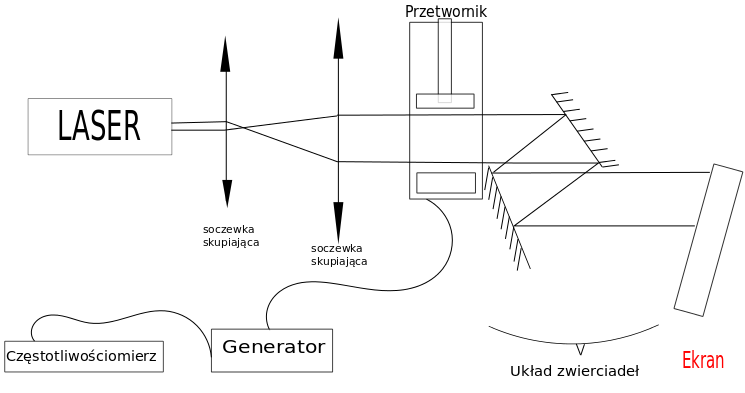
\includegraphics[width = 15cm]{Rysunek.png}
%    \caption{Układ pomiarowy}
%  \end{center}
%\end{figure}


\section{Cel ćwiczenia}

Celem naszego ćwiczenia projektowego było naprawienie ogniwa metanolowego. Ogniwo, które otrzymaliśmy miało bardzo niską sprawność i można było z niego pobierać moc rzędu wielkości mikro Watów.



\section{Wstęp}

Ogniwo z jakim mieliśmy do czynienia nazywa się Direct Methanol Fuel Cell - paliwem w nim jest metanol.

Podstawowym wyznacznikiem naprawienia ogniwa, było to, żeby mogło zasilać dołączony do niego wiatraczek.

Ważnymi parametrami ogniwa są:
\begin{itemize}
\item oporność wewnętrzna
\item moc
\item napięcie maksymalne
\end{itemize}
\section{Użyty sprzęt i układy pomiarowe}

W naszym ćwiczeniu używaliśmy:
\begin{itemize}
\item komputera
\item metanolu i kwasu siarkowego VI
\item mierników uniwersalnych
\item oporników dekadowych
\item wagi precyzyjnej
\end{itemize}

\section{Przebieg ćwiczenia}

Na początku zmierzyliśmy charakterystyki ogniwa dla róznych zawartości metanolu w paliwie:

Tu wrzucimy wykresy z pierwszego sheet'a w gnumericu expotent

By zwiększyć wydajność ogniwa wykonaliśmy na nim różne zabiegi:
\begin{itemize}
\item zwilżanie membrany (nafionowej)
\item ogrzewanie
\item kolejne cykle z nowym paliwem
\item "kąpiel" w rozcięczonym kwasie siarkowym VI
\end{itemize}

Zwilżanie membrany polepsza parametry ogniwa. Musi być jednak wykonane w odpowiedni sposób. Najlepszym ze sprawdzonych przez nas sposobów było 'chuchanie'.

Największy jednak wpływ na parametry ogniwa miały kolejne cykle z nowym paliwem. Każde kolejne badanie charakterystyk pokazywało, że wydajność wzrasta.

Bardzo dobry skutek na ogniwo wywarła "kąpiel" w rozcięczonym kwasie siarkowym VI.

Tu przedstawiamy charakterystyki ogniw po naszych zabiegach:

Kolejne obrazki z gnumerica...

Interesowały nas także charakterystyki zużycia paliwa i napięcia od czasu.

Zmierzyliśmy takie charakterystyki dla trzech wartości zawartości paliwa: $3\%$, $2\%$, i $1\%$

\begin{figure} [H]
 \begin{center}
    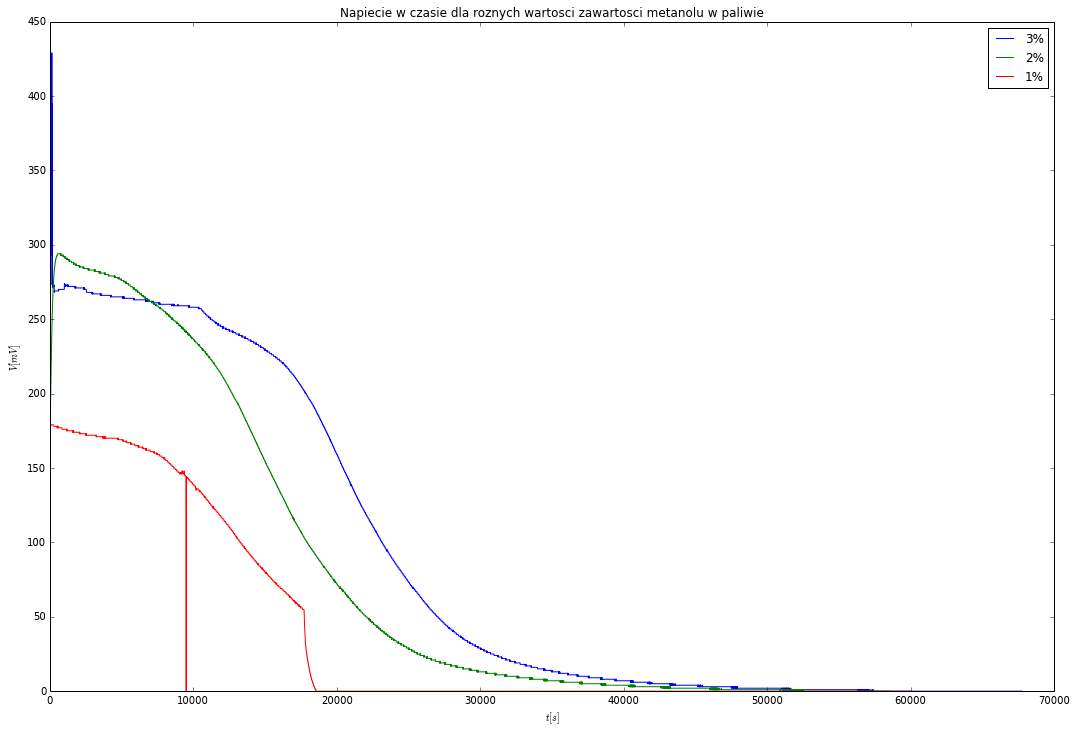
\includegraphics[width = 15cm]{DMFC_U(T).png}
    \caption{Układ pomiarowy}
  \end{center}
\end{figure}


\section{Opracowanie wyników}


\section{Wnioski}
Udało nam się przywrócić ogniwo do pełnej sprawności i dobrze je zcharakteryzować.

\end{document}
